\documentclass[12pt,a4paper,utf8]{ctexart}
\usepackage{graphicx}
\usepackage{amsmath}
\usepackage{amssymb}
\usepackage{subfig}
\usepackage{cite}
\usepackage[ntheorem]{empheq}
\usepackage{enumitem}
\usepackage{fullpage}
\usepackage{cleveref}
\usepackage{cellspace}
\usepackage{listings}
\usepackage{color}
\usepackage{algorithm}  
\usepackage{algorithmicx}  
\usepackage{algpseudocode}  
\definecolor{gray}{rgb}{0.5,0.5,0.5}
\definecolor{dkgreen}{rgb}{.068,.578,.068}
\definecolor{dkpurple}{rgb}{.320,.064,.680}
\usepackage{lipsum}

\makeatletter
\newenvironment{breakablealgorithm}
  {% \begin{breakablealgorithm}
   \begin{center}
     \refstepcounter{algorithm}% New algorithm
     \hrule height.8pt depth0pt \kern2pt% \@fs@pre for \@fs@ruled
     \renewcommand{\caption}[2][\relax]{% Make a new \caption
       {\raggedright\textbf{\ALG@name~\thealgorithm} ##2\par}%
       \ifx\relax##1\relax % #1 is \relax
         \addcontentsline{loa}{algorithm}{\protect\numberline{\thealgorithm}##2}%
       \else % #1 is not \relax
         \addcontentsline{loa}{algorithm}{\protect\numberline{\thealgorithm}##1}%
       \fi
       \kern2pt\hrule\kern2pt
     }
  }{% \end{breakablealgorithm}
     \kern2pt\hrule\relax% \@fs@post for \@fs@ruled
   \end{center}
  }
\makeatother

\floatname{algorithm}{算法}  
\renewcommand{\algorithmicrequire}{\textbf{输入:}}  
\renewcommand{\algorithmicensure}{\textbf{输出:}}  

% set Matlab styles
\lstset{
   language=Matlab,
   keywords={break,case,catch,continue,else,elseif,end,for,function,
      global,if,otherwise,persistent,return,switch,try,while},
   basicstyle=\ttfamily,
   keywordstyle=\color{blue}\bfseries,
   commentstyle=\color{dkgreen},
   stringstyle=\color{dkpurple},
   backgroundcolor=\color{white},
   tabsize=4,
   showspaces=false,
   showstringspaces=false
}

\begin{document}
\CJKfamily{zhkai}	


\begin{center}
\textbf{计算方法 作业一}\\
\textbf{姓名 ~范文~~~~~~~~ 学号 ~PB18111679~~~~~~ 日期 2021.5.6}\\
\end{center}

\begin{center}
\fbox{
\begin{minipage}{40em}
\vspace{5cm}
\hspace{20cm}
\end{minipage}}
\end{center}
\vspace{1cm}

\paragraph{实验环境}
\subparagraph{硬件配置}
        8个Intel(R) Core(TM) i5-8250U核,内存8G,交换区8G
\subparagraph{操作系统}
        ubuntu 20.04,内核版本为5.4.0-72-generic
\subparagraph{Matlab}
        MATLAB R2016b 

\begin{enumerate}
\item[第一题] \textbf{线性方程组求解}

    \begin{itemize}
    \item [(a)] \textbf{使用Jacobi和Gauss-Siedel方法求解}
    \par
    首先,我使用了Jacobi迭代方法,迭代中使用矩阵运算x\_next = R*x\_cur + g,并设置误差为$10^{-15}$,其Matlab代码如下:
\begin{lstlisting}[frame=single]
% implementing jacobi iteration
% @A: the coefficent matrix on LHS
% @b: the constant matrix on RHS
% @x_exact: the exact solution to this equation set
% @epsilon: the error bound
% @max_loop: the maximal number of loops
% print the info during each iteration
% and plot the error in each iteration
function jacobi_solution(A,b,x_exact,epsilon,max_loop)
    [A_row,A_col] = size(A);
    [b_row,~] = size(b);
    % check whether the dimension of A and b matches.
    if(A_row ~= b_row)
        fprintf('A and b''s dim doesn''t match.\n');
        return;
    end
    
    % -------------------------------------------------
    % X(k+1) = RX(k) + g
    % -------------------------------------------------
    
    % x_cur is the solution of the current step of loop
    % x_cur is initialized as a vector full of 0
    x_cur = zeros(A_col,1);
    
    % x_next is the solution of the next step of loop
    % x_cur is initialized as a vector full of 1
    x_next = ones(A_col,1);
    
    % the error between current solution 
    % and exact solution in each loop
    error = zeros(A_col,1);
    % an vector to store the infinite norm 
    % of errors in each iteration
    error_list = zeros(max_loop,1);
    
    % R is the factor matrix in the loop
    % when i != j, R(i,j) = -A(i,j)/A(i,i)
    R = zeros(size(A));
    for i = 1:A_row
        for j = 1:A_col
            if i ~= j
                R(i,j) = -A(i,j)/A(i,i);
            end
        end
    end
    
    % g is the matrix to be added in each iteration
    % gi = bi/aii
    g = b;
    for i = 1:b_row
        g(i,1) = b(i,1)/A(i,i);
    end
    
    % show the items for the output info
    % x_size means the number of variables
    [x_size,~] = size(x_exact);
    % loop time
    loop = 0;
    % main iteration
    while( norm(x_cur-x_next,inf) > epsilon ...
            && loop <= max_loop )
        loop = loop + 1;
        % update x_cur
        x_cur = x_next;
        % update x_next
        x_next = R*x_cur + g;
        % record the error
        error = x_exact - x_cur;
        error_list(loop,1) = norm(error,inf);
        % print the information of each loop
        print_info(loop,x_cur,error);
    end
    % plot the max errors in each iteration
    semilogy(error_list);
    hold on;
end
\end{lstlisting}
    \par
    然后,我使用了Gauss-Siedel迭代方法,迭代中使用矩阵运算x\_next = S*x\_cur + f;,并设置误差为$10^{-15}$,其Matlab代码如下:
\begin{lstlisting}[frame=single]
% implementing jacobi iteration
% @A: the coefficent matrix on LHS
% @b: the constant matrix on RHS
% @x_exact: the exact solution to this equation set
% @epsilon: the error bound
% @max_loop: the maximal number of loops
% print the info during each iteration
function gauss_siedel_solution(A,b,x_exact,epsilon,max_loop)
    [A_row,A_col] = size(A);
    [b_row,~] = size(b);
    % check whether the dimension of A and b matches.
    if(A_row ~= b_row)
        fprintf('A and b''s dim doesn''t match.\n');
        return;
    end
    
    % -------------------------------------------------
    % originally, it should be
    % X(k+1) = SX(k) + f
    % where S = -(D+L)_inv U and f = -(D+L)_inv b
    % -------------------------------------------------
    
    % x_cur is the solution of the current loop
    % x_cur is initialized as a vector full of 0
    x_cur = zeros(A_col,1);
    
    % x_next is the solution of the next loop
    % x_cur is initialized as a vector full of 1
    x_next = ones(A_col,1);
    
    % D is the diagnal matrix of A
    D = diag(diag(A));
    
    % L is the lower triangle matrix of A
    L = tril(A,-1);
    
    % U is the upper triangle matrix of A
    U = triu(A,1);
    
    inv_D_plus_L = inv(D+L);
    S = -inv_D_plus_L * U;
    f = inv_D_plus_L * b;
    % show the items for the output info
    % x_size means the number of variables
    [x_size,~] = size(x_exact);
    
    % the error between current solution 
    % and exact solution in each loop
    error = zeros(A_col,1);
    % an vector to store the infinite norm 
    % of error in each iteration
    error_list = zeros(max_loop,1);
    
    % loop time
    loop = 0;
    % main iteration
    while( norm(x_cur-x_next,inf) > epsilon ...
                && loop < max_loop )
        loop = loop + 1;
        % update the current solution
        x_cur = x_next;
        % get the next solution
        x_next = S*x_cur + f;
        % record the error
        error = x_exact - x_cur;
        error_list(loop,1) = norm(error,inf);
        % show the info during each loop
        print_info(loop,x_cur,error);
    end
    % plot the max errors in each iteration
    semilogy(error_list);
    hold on;
end
\end{lstlisting}
    \par
    因此,得到了两个算法误差的semilogy图如图1所示.这里横坐标表示迭代次数,纵坐标表示中间解与精确解的误差中分量最大的值.实际上,Jacobi算法迭代了830次才停止,而Gauss-Siedel算法迭代了394次就停止了.从图1也可以看出Gauss-Siedel算法在本题目中收敛更快.
    \begin{figure}[htbp]
		\centering
		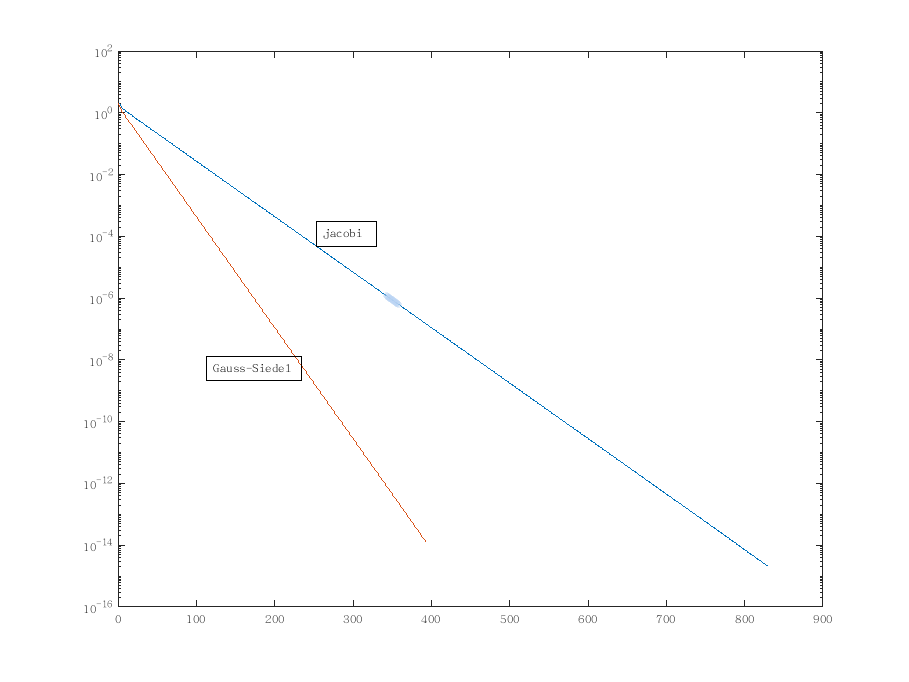
\includegraphics[scale=0.6]{pictures/jacobi_gauss_siedel.png}
		\caption{\small{Jacobi及Gauss-Siedel算法收敛速度的semilogy图}} %图1
    \end{figure}

    \item [(b)] \textbf{使用SOR松弛方法求解}
    我使用了SOR松弛方法求解,也是设置误差为$10^{-15}$,并令松弛因子 $\omega = 0.9,0.8,0.6,0.5$,得到了迭代误差随迭代次数的semilogy图如图2所示.其中,Matlab代码如下:
\begin{lstlisting}[frame=single]

% implementing SOR iteration
% @A: the coefficent matrix on LHS
% @b: the constant matrix on RHS
% @w: the relaxation factor
% @x_exact: the exact solution to this equation set
% @epsilon: the error bound
% @max_loop: the maximal number of loops
% print the info during each iteration
function SOR_solution(A,b,w,x_exact,epsilon,max_loop)
    [A_row,A_col] = size(A);
    [b_row,~] = size(b);
    % check whether the dimension of A and b matches.
    if(A_row ~= b_row)
        fprintf('A and b''s dim doesn''t match.\n');
        return;
    end
    % check whether w is out of valid bound
    if(w < 0)
        fprintf('w should be positive.\n');
        return;
    end
    
    % -------------------------------------------------
    % X(k+1) = Sw*X(k) + f
    % -------------------------------------------------
    
    % x_cur is the solution of the current loop
    % x_cur is initialized as a vector full of 0
    x_cur = zeros(A_col,1);
    
    % x_next is the solution of the next loop
    % x_cur is initialized as a vector full of 1
    x_next = ones(A_col,1);
    
    % D is the diagnal matrix of A
    D = diag(diag(A));
    % temp result to calculate Sw and f
    w_D_inv = w*inv(D);
    
    % L is the lower triangle matrix of A
    L = tril(A,-1);
    
    % U is the upper triangle matrix of A
    U = triu(A,1);
    
    % I is identity matrix
    I = eye(A_col);
    
    % temp result to calculate Sw and f
    temp = inv(I + w_D_inv * L);
    
    % Sw is the factor matrix in the loop
    Sw = temp *( (1-w) * I - w_D_inv * U );
    
    % f is the matrix to be added in each iteration
    f = temp * w_D_inv * b;
    
    % the error between current solution 
    % and exact solution in each loop
    error = zeros(A_col,1);
    % an vector to store the infinite 
    % norm of errors in each iteration
    error_list = zeros(max_loop,1);
    
    % show the items for the output info
    % x_size means the number of variables
    [x_size,~] = size(x_exact);
    % the row of items(such as loop time,option,variables)
    fprintf('  loop    option    ');
    for i = 1:x_size
        fprintf('  x%d      ',i);
    end
    fprintf('\n');
    
    % loop time
    loop = 0;
    % main iteration
    while( norm(x_cur-x_next,inf) > epsilon ...
            && loop < max_loop)
        loop = loop + 1;
        %semilogy(loop,norm(x_cur-x_next,inf));
        x_cur = x_next;
        x_next = Sw*x_cur + f;
        % record the error
        error = x_exact - x_cur;
        error_list(loop,1) = norm(error,inf);
        % show the info during each loop
        print_info(loop,x_cur,error);
    end
    % plot the max errors in each iteration
    semilogy(error_list);
    hold on;
end
\end{lstlisting}
    \par
    图2中,这里横坐标表示迭代次数,纵坐标表示中间解与精确解的误差中分量最大的值. 
    \par
    由图2可知,当松弛因子$\omega < 1$时,SOR收敛速度随着松弛因子$\omega$减小而减慢.当松弛因子 $\omega = 0.9$ 时,SOR方法收敛速度接近于Gauss-Siedel算法的收敛速度;随着$\omega$的减小,SOR方法的收敛速度逐渐变慢. 当$\omega = 0.6$时,SOR方法的收敛速度开始满于Jacobi算法的收敛速度.
    \par
    松弛因子$\omega > 1$时,SOR收敛速度随着松弛因子$\omega$增大而先增大再减小.由图2知,使得收敛速度最快的松弛因子$\omega$处于$[1.5,1.7]$范围内.当$\omega = 1.6$时,迭代只需要最少的161步.
    \par
    因此,当 $\omega = 1.6$ 时,SOR方法达到了最快收敛速度.
    \begin{figure}[htbp]
        \centering
        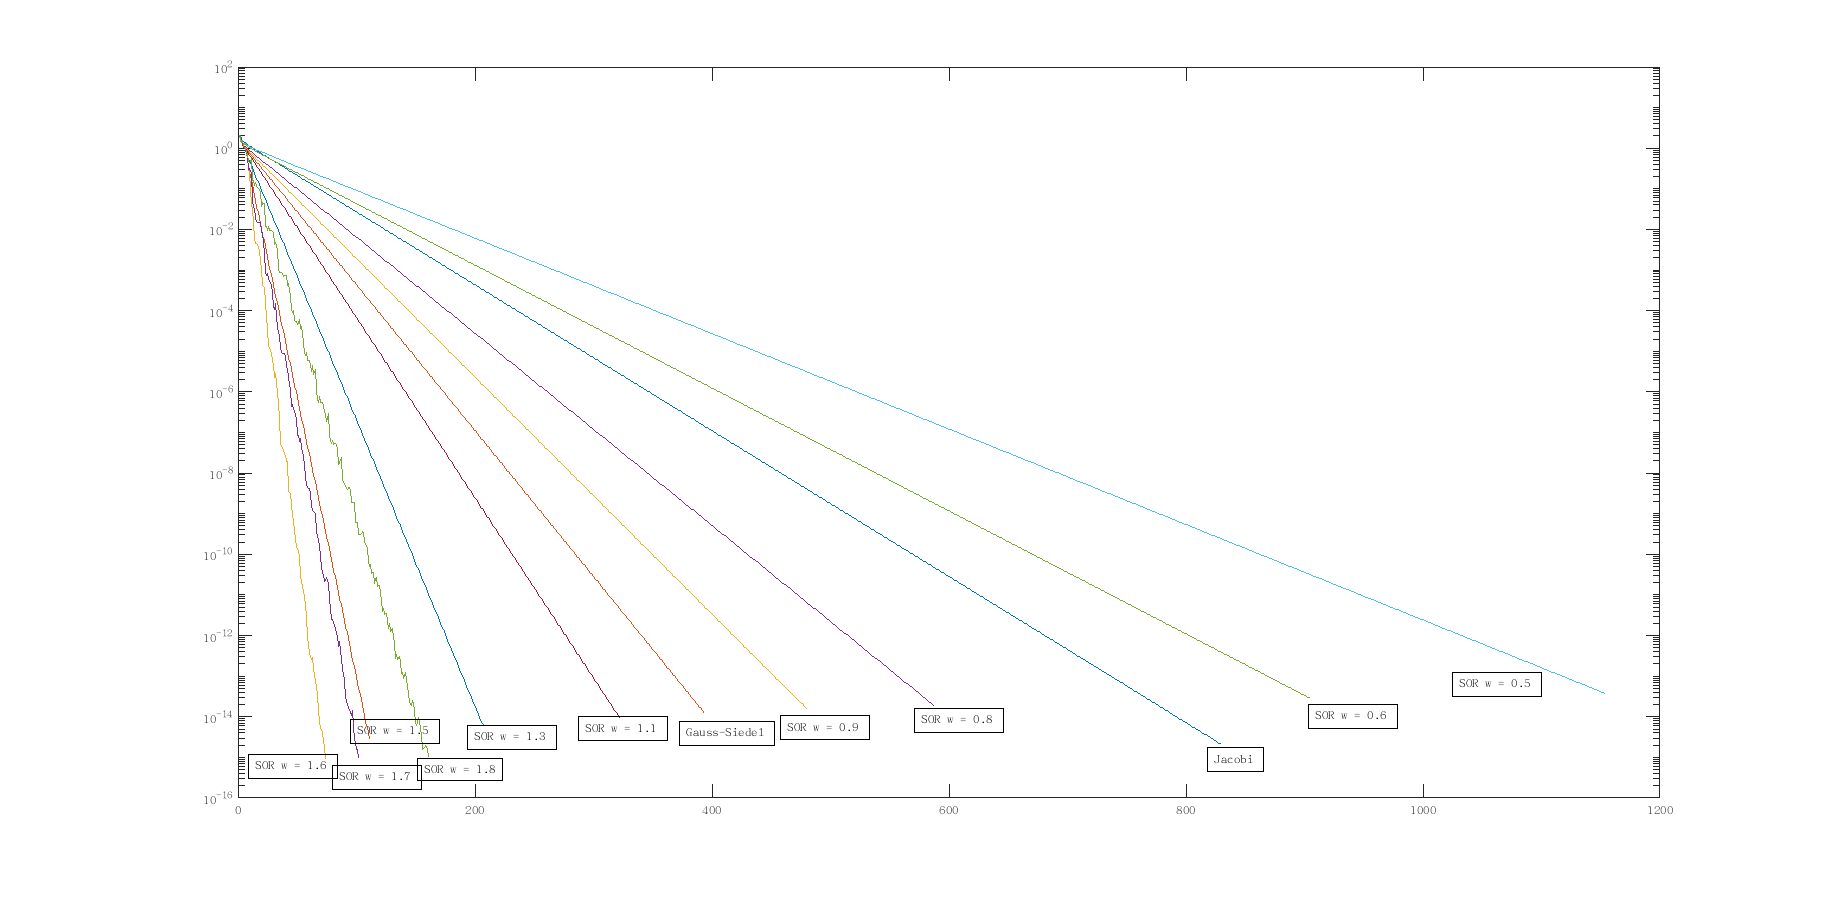
\includegraphics[scale=0.4]{pictures/all.png}
        \caption{\small{Jacobi,Gauss-Siedel和SOR算法收敛速度的semilogy图}} %图2
    \end{figure}
    
    \item [(c)] \textbf{稀疏矩阵的优化}
    \par
    这里,我对以上三种算法的迭代进行优化.在原有算法中,使用矩阵乘法来更新解,即x\_next = M*x\_cur + N;由于原矩阵$A$是一个较大的稀疏矩阵,因此可以把乘法展开成循环,从而将其优化.比如,我们可以知道在$A$的第$i$行中,只有第$i-1$到$i+1$列的元素非零,因此可以只用考虑这些非零元素,从而减少运算量.
    \par
    Jacobi方法优化后的迭代关键代码如下所示:
\begin{lstlisting}[frame=single]
% loop time
loop = 0;
% main iteration
while(norm(x_cur-x_next,inf)>epsilon && loop<=max_loop)
    loop = loop + 1;
    % update x_cur
    x_cur = x_next;
    % update x_next by a loop
    for i = 1:A_row
        sum = 0;
        for j = max(i-1,1):min(i+1,A_col)
            sum = sum + A(i,j)*x_cur(j,1);
        end
        x_next(i,1)=(b(i,1) - sum)/A(i,i)+x_cur(i,1); 
    end
        
    % record the error
    error = x_exact - x_cur;
    error_list(loop,1) = norm(error,inf);
end
\end{lstlisting}
    Gauss-Siedel方法优化后的迭代关键代码如下所示:
\begin{lstlisting}[frame=single]
% loop time
loop = 0;
% main iteration
while( norm(x_cur-x_next,inf) > epsilon ...
        && loop < max_loop )
    loop = loop + 1;
    % update the current solution
    x_cur = x_next;
    % get the next solution 
    for i = 1:x_size
        sum = 0;
        for j = max(i-1,1):min(i+1,x_size)
            sum = sum + A(i,j)*x_next(j,1);
        end
        x_next(i,1)=(b(i,1)-sum)/A(i,i)+x_next(i,1);
    end
    % show the info during each loop
    %print_info(loop,x_cur,x_exact);
end
\end{lstlisting}
    SOR方法优化后的迭代关键代码如下所示:
\begin{lstlisting}[frame=single]
% loop time
loop = 0;
% main iteration
while( norm(x_cur-x_next,inf) > epsilon ...
        && loop < max_loop)
    loop = loop + 1;
    x_cur = x_next;
    % update x_next with opt to sparse matrix A
    for i = 1:A_row
        sum_1 = 0;
        sum_2 = 0;
        if(i > 1)
            sum_1 = A(i,i-1)*x_next(i-1,1);
        end
        if(i < A_row)
            sum_2 = A(i,i+1)*x_cur(i+1,1);
        end
        x_temp(i,1) = (b(i,1) - sum_1 - sum_2)/A(i,i);
        x_next(i,1) = w*x_temp(i,1) + (1-w)*x_cur(i,1);
    end
    % record the error
    error = x_exact - x_cur;
    error_list(loop,1) = norm(error,inf);
end
\end{lstlisting}
    \par
    分别测试优化前后的三种算法,每次测试中运行算法11次且只统计后10次运行的时间和,得到了它们时间的对比如下:
\begin{lstlisting}
>> Jacobi
830     
value   1.000000000000001   0.000000000000001   
        1.000000000000002   0.000000000000001   
        0.000000000000002   0.000000000000001   
        0.000000000000002  -0.999999999999999   
        0.000000000000001  -1.000000000000000
          
calling original Jacobi for 10 times, 
sum time = 0.049108s
--------------------------------------------------
>> Jacobi_opt
833     
value   1.000000000000000   0.000000000000001   
        1.000000000000001   0.000000000000002   
        0.000000000000001   0.000000000000002   
        0.000000000000001  -0.999999999999998   
        0.000000000000001  -0.999999999999999
          
calling optimized Jacobi for 10 times, 
sum time = 0.017911s
--------------------------------------------------
>> Gauss_Siedel
394     
value   1.000000000000004   0.000000000000007   
        1.000000000000010   0.000000000000011   
        0.000000000000012   0.000000000000011   
        0.000000000000010  -0.999999999999992   
        0.000000000000006  -0.999999999999997

calling original Gauss-Siedel for 10 times,
sum time = 0.029954s
--------------------------------------------------
>> Gauss_Siedel_opt
395     
value   1.000000000000004   0.000000000000007   
        1.000000000000009   0.000000000000011   
        0.000000000000011   0.000000000000011   
        0.000000000000009  -0.999999999999992   
        0.000000000000005  -0.999999999999997

calling optimize Gauss-Siedel for 10 times,
sum time = 0.008248s
--------------------------------------------------
>> SOR
588     
value   1.000000000000006   0.000000000000011
        1.000000000000015   0.000000000000017   
        0.000000000000018   0.000000000000018   
        0.000000000000016  -0.999999999999987   
        0.000000000000009  -0.999999999999995

calling original SOR with w = 0.800000 for 10 times,
sum time = 0.018574s
--------------------------------------------------
>> SOR_opt
589     
value   1.000000000000006   0.000000000000010
        1.000000000000014   0.000000000000016   
        0.000000000000017   0.000000000000017   
        0.000000000000015  -0.999999999999988   
        0.000000000000008  -0.999999999999996

calling optimized SOR with w = 0.800000 for 10 times,
sum time = 0.013638s
--------------------------------------------------
>>  
\end{lstlisting}
    \par
    由于使用矩阵运算和循环展开的计算方法不同,因此会在每一步带来一定的误差,导致最终结果和迭代次数会略有不同.
    前后对比可知,在同一精度下结果几乎一样,迭代次数几乎一样的情况下,
    优化后的Jacobi算法的运行时间(0.017911s)只有原来运行时间(0.049108s)的三分之一左右,
    优化后的Gauss-Siedel算法的运行时间(0.008248s)只有原来运行时间(0.029954s)的三分之一左右,
    优化后的SOR算法($\omega = 0.8$)的运行时间(0.013638)只有原来运行时间(0.018574s)的三分之二左右.
    因此,三个算法都实现了优化.前两个算法的优化力度较大,后一个算法的优化力度较小.
    \par
    实际上,本次优化的缺点是,它只能针对特定的输入矩阵$A$进行优化:
    如果$A$的非零元素的分布有所变化,则需要重新写一个新的优化算法.
    我还自己写了一个用三元组优化稀疏矩阵乘法的算法,
    但是,自己写的函数肯定没法和Matlab的矩阵乘法库函数相比.
    对比的成果是,对于输入为的10维稀疏矩阵的Gauss-Siedel算法,
    Mablab矩阵乘法(用时0.021245s)比我自己写的稀疏矩阵乘法(用时1.571271s)快两个数量级.
    \par
    看来,我们不能天真地以为自己写一点矩阵的优化,就能打败Matlab成熟的库函数.
\begin{lstlisting}
>> Gauss_Siedel
--------------------------------------------------
394     
value   1.000000  0.000000  1.000000  0.000000  0.000000       
        0.000000  0.000000 -1.000000  0.000000 -1.000000
error   0.000000  0.000000  0.000000  0.000000  0.000000  
        0.000000  0.000000  0.000000  0.000000  0.000000
calling original Gauss-Siedel for 10 times, 
sum time = 0.021245s
>> sm_Gauss_Siedel
--------------------------------------------------
394     
value   1.000000  0.000000  1.000000  0.000000  0.000000  
        0.000000  0.000000 -1.000000  0.000000 -1.000000
error   0.000000  0.000000  0.000000  0.000000  0.000000  
        0.000000  0.000000  0.000000  0.000000  0.000000
calling sparse-matrix Gauss-Siedel for 10 times, 
sum time = 1.571271s
\end{lstlisting}
    \end{itemize}

\item[第二题] \textbf{Newton迭代法}
    \begin{itemize}
    \item[(a)] \textbf{实现Newton迭代法}
    \par
    Newton迭代法的关键代码如下:
\begin{lstlisting}[frame=single]
% use Newton iteration to get the solution
% of f(x) = 0 where left <= x <= right
% print the info of temporary solution 
% and error during each interation
% @left: left boundary of the solution
% @right: right boundary of the solution
% @f: the consecutive real function
% @max_loop: maximal number of loops
% @epsilon: the error bound in this range
function newton_solution(left,right,f,max_loop,epsilon)
    % x_last is the solution in the last iteration
    x_last = (left + right)/2;
    % x_cur is the solution in the current iteration
    x_cur = 1;
    % f's differential
    diff_f = diff(f);
    % error in this loop
    error = 0;
    % the vector to store errors in each iteration
    errors = zeros(max_loop,1);
    % the evaluated order in iteration
    order = 0;
   
    % print the info
    dash_str = repmat('-', 1, 50);
    fprintf('%s\n',dash_str);
    display(f);
    fprintf('looking for a root in [%f,%f]\n',left,right);
    fprintf('  loop        x         error       order\n');
    
    % main loop
    for loop = 1:max_loop
        % set x_cur = x_last - f(x_last)/f'(x_last)
        x_cur = x_last - subs(f,symvar(f),x_last)...
            /subs(diff_f,symvar(diff_f),x_last);
        error = abs(x_cur - x_last);
        errors(loop,1) = error;
        % print the current solution, current log error 
        % and approximate order
        fprintf('%5d    %10f    %10f',loop,x_cur,error);
        if(loop >= 3)
            order = log(errors(loop,1)/errors(loop-1,1)) ...
                    / log(errors(loop-1,1)/errors(loop-2,1));
            fprintf('  %10f\n',order);
        else
            fprintf('\n');
        end
        if( abs(x_cur - x_last) < epsilon )
            break;
        else
            x_last = x_cur;
        end
    end
    fprintf('at last, the solution is x = %10f\n',x_cur);
end
\end{lstlisting}
    在这里,我设置的误差为$10^{-6}$,且迭代初始值为区间的中点.之后,运行这个算法,在三个区间求根的过程中,得到了每一步迭代的近似值如下所示.
\begin{lstlisting}
--------------------------------------------------
looking for a root in [-3.000000,0.000000]
  loop        x         error       order
    1     -0.984127      0.515873
    2     -0.773163      0.210964
    3     -0.733438      0.039725    1.867308
    4     -0.732052      0.001385    2.009971
    5     -0.732051      0.000002    2.003883
    6     -0.732051      0.000000    2.000079
at last, the solution is x =  -0.732051
--------------------------------------------------
looking for a root in [0.000000,2.000000]
  loop        x         error       order
    1      1.000000      0.000000
at last, the solution is x =   1.000000
--------------------------------------------------
looking for a root in [2.000000,4.000000]
  loop        x         error       order
    1      2.777778      0.222222
    2      2.733757      0.044021
    3      2.732053      0.001703    2.008705
    4      2.732051      0.000003    2.004356
    5      2.732051      0.000000    2.000100
at last, the solution is x =   2.732051
\end{lstlisting}
    \par    
    因此,得到了这三个根的近似值为$x_l = -0.732051, x_m = 1.000000, x_r = 2.732051.$

    \item[(b)] \textbf{估计Newton迭代法的收敛阶数}
    \par
    在Newton迭代中,设$e_i$表示第$i$次迭代后的误差 $\alpha$为收敛阶数.
    则有 $ \left| e_{i+1} \right|  \approx \lambda { \left| e_{i} \right|} ^ \alpha$,
    $ \left| e_{i} \right|  \approx \lambda {\left| e_{i-1} \right|} ^ \alpha$.
    所以,$\alpha \approx \frac{ \log{ \left| \frac{e_{i+1}}{e_i} \right|} }
        { \log{ \left| \frac{e_{i}}{e_{i-1}} \right|} }$
    \par
    由因为我们没法知道精确解,因此使用每轮迭代中估计出来的解进行代替,即
    $\alpha \approx \frac{ \log{ \left| \frac{ x_{n+1} - x_n }{x_n - x_{n-1}} \right|} }
        { \log{ \left| \frac{x_n - x_{n-1}}{x_{n-1} - x_{n-2}} \right|} }$.
    所以,我们需要三轮迭代的结果才能得到一个收敛阶数的估计值.
    \par
    在Matlab代码中,我用一个向量
    errors来存放每一轮迭代后算出的误差,并在第三轮迭代之后利用
\begin{lstlisting}
order = log(errors(loop,1)/errors(loop-1,1)) ...
            / log(errors(loop-1,1)/errors(loop-2,1));
\end{lstlisting}
    来估计收敛阶数.
    因此,每轮估计的的收敛阶数在本题(a)中结果的最右边一行中展示.去掉第一次迭代开始时偏离较大的1.867308,计算其他估计值的算数平均值,得到Newton迭代算法收敛阶数$\alpha \approx 2.0045$.

    \item[(c)] \textbf{收敛阶数的误差分析}
    \par 
    收敛阶数的估计值$\alpha \approx 2.0045 > 2$.这里是由于估计的时候是使用迭代的估计解来计算每一轮的误差,而非使用精确解来计算每一轮的误差.在我运行的程序中,Newton迭代法总是在精确解的一侧不断逼近,这是因为:
    \par
    在区间$[-3,0]$上,迭代的初始值为$x_0 = -1.5 < x_l = -0.732051$.由于$f$在$[-3,0]$上是凸单调递增的,因此之后每一轮迭代的解$x_i < x_l$;
    在区间$[0,2]$上,迭代的初始值为$x_0 = 1$,恰好在误差范围内等于$x_m$,因此迭代直接结束;
    在区间$[2,4]$上,迭代的初始值为$x_0 = 3 > x_r = 2.732051$.由于$f$在$[2,4]$是凹单调递增的,因此之后每一轮迭代的解$x_i > x_r$.
    \par
    因此相邻两轮迭代之间的误差肯定小于迭代结果和精确解之间的误差,所以计算收敛阶数时,使用的误差更小.所以,得到的收敛阶数更大.
    \end{itemize}

\item[第三题] \textbf{求矩阵特征值和特征向量}
    \begin{itemize}
    \item[(a)] \textbf{设计幂法的伪代码}
    \par 为了能够解决书上168页中的三种情况(只有一个正的按模分量最大的特征值,只有一个负的按模分量最大的特征值,有两个互为相反数的按模分量最大的特征值),根据徐老师上课展示的代码,我的伪代码如算法1所示:
    \begin{algorithm}  
        \caption{Power method}  
        \begin{algorithmic}[1] %每行显示行号  
            \Require 方阵$A$, 最大迭代次数$max\_loop$,误差界限$\epsilon$
            \Ensure 按模最大的特征值$lambda$及其对应的特征向量$q$
            \Function {Power\_method}{$A,max\_loop,\epsilon$}  
                \State $q\_last$ 代表上一次迭代的特征向量.
                \State $q\_odd\_last$ 代表上一次奇数次迭代的特征向量.
                \State $q\_even\_last$ 代表上一次偶数次迭代的特征向量.
                \State $q\_cur$ 代表这一次迭代的特征向量.
                \State $q\_norm\_cur$ 代表这一次迭代的规范化的特征向量.
                \State $q\_odd\_cur$ 代表这一次奇数次迭代的特征向量.
                \State $q\_even\_cur$ 代表这一次偶数次迭代的特征向量.
                \State $\lambda$ 代表特征值
                \For{$loop = 1:max\_loop$}
                    \State $q\_cur = A*q\_last$; // 更新这一次迭代的特征向量
                    \State // 对特征向量进行规范化处理并进行保存
                    \State $\lambda \gets q\_cur$中模最大的元素;
                    \State $q\_norm\_cur = q\_cur / \lambda $;
                    \If{$loop$为奇数}
                        $q\_odd\_cur = q\_norm\_cur$;
                    \Else{}
                        $q\_even\_cur = q\_norm\_cur$;
                    \EndIf
                    \State //(1) $X^{(k)}$收敛,则只有一个正的模最大的特征值
                    \If{ ${ \Vert q\_norm\_cur - q\_last \Vert}_{\infty} < \epsilon$}
                        \Return{$\lambda,q\_norm\_cur$}
                    \EndIf
                    \State //(2) $X^{(2k)},X^{(2k+1)}$收敛到反号的向量,则只有一个负的模最大的特征值
                    \If{${ \Vert q\_norm\_cur + q\_last \Vert}_{\infty} < \epsilon$}
                        \Return{$-\lambda,q\_norm\_cur$}
                    \EndIf
                    \State //(3) $X^{(2k)},X^{(2k+1)}$收敛到不同的向量,则有两个异号的模最大的特征值
                    \If{${ \Vert q\_odd\_cur - q\_odd\_last \Vert}_{\infty},{ \Vert q\_even\_cur - q\_even\_last \Vert}_{\infty} < \epsilon$}
                        \State $q\_next = A * q\_cur$;
                         $\lambda = \sqrt{ q\_next(1) / q\_last(1) }$;
                        \State $q\_1 = q\_next + \lambda * q\_cur$;
                         $q\_1 = q\_1 / {\Vert q\_1 \Vert}_{\infty}$;
                        \State $q\_2 = q\_next - \lambda * q\_cur$;
                        $q\_2 = q\_2 / {\Vert q\_2 \Vert}_{\infty}$;
                        \State \Return{$\lambda,q\_1;-\lambda,q\_2$}
                    \EndIf
                    \State // 为下一次迭代更新上一次迭代的特征向量
                    \If{$loop$为奇数}
                        $q\_odd\_last = q\_norm\_cur$;
                    \Else{}
                        $q\_even\_last = q\_norm\_cur$;
                    \EndIf
                    \State $ q\_last = q\_norm\_cur$;
                \EndFor 
                \State \Return{$NAN,null$} // 在$max\_loop$步数内没有收敛,返回空.
            \EndFunction  
        \end{algorithmic}  
    \end{algorithm}  
    
    \item[(b)] \textbf{求解按模最大的特征值和对应的特征向量}
    \par
    我使用Matlab程序实现上述幂法,并设置误差上界为$10^{-15}$,用于求解$A$的模最大的特征值和特征向量.则得到了迭代中每一步的$\lambda$和$q\_cur$如下所示:
    \begin{lstlisting}
>> power_method
loop    eigenvalue     eigenvector
1     1316.000000    (-0.306231  1.000000  -0.782675  0.113222 )
2     7.475684    (-0.307888  1.000000  -0.789998  0.123907 )
3     7.005286    (-0.308990  1.000000  -0.792478  0.131185 )
4     7.372036    (-0.309702  1.000000  -0.793094  0.135043 )
5     7.692634    (-0.310069  1.000000  -0.793170  0.136776 )
6     7.867047    (-0.310233  1.000000  -0.793148  0.137484 )
7     7.946022    (-0.310301  1.000000  -0.793125  0.137761 )
8     7.978802    (-0.310328  1.000000  -0.793113  0.137867 )
9     7.991825    (-0.310338  1.000000  -0.793107  0.137907 )
10     7.996880    (-0.310342  1.000000  -0.793105  0.137922 )
11     7.998817    (-0.310344  1.000000  -0.793104  0.137928 )
12     7.999553    (-0.310344  1.000000  -0.793104  0.137930 )
13     7.999832    (-0.310345  1.000000  -0.793104  0.137931 )
14     7.999937    (-0.310345  1.000000  -0.793103  0.137931 )
15     7.999976    (-0.310345  1.000000  -0.793103  0.137931 )
16     7.999991    (-0.310345  1.000000  -0.793103  0.137931 )
17     7.999997    (-0.310345  1.000000  -0.793103  0.137931 )
18     7.999999    (-0.310345  1.000000  -0.793103  0.137931 )
19     8.000000    (-0.310345  1.000000  -0.793103  0.137931 )
20     8.000000    (-0.310345  1.000000  -0.793103  0.137931 )
21     8.000000    (-0.310345  1.000000  -0.793103  0.137931 )
22     8.000000    (-0.310345  1.000000  -0.793103  0.137931 )
23     8.000000    (-0.310345  1.000000  -0.793103  0.137931 )
24     8.000000    (-0.310345  1.000000  -0.793103  0.137931 )
25     8.000000    (-0.310345  1.000000  -0.793103  0.137931 )
26     8.000000    (-0.310345  1.000000  -0.793103  0.137931 )
27     8.000000    (-0.310345  1.000000  -0.793103  0.137931 )
28     8.000000    (-0.310345  1.000000  -0.793103  0.137931 )
29     8.000000    (-0.310345  1.000000  -0.793103  0.137931 )
30     8.000000    (-0.310345  1.000000  -0.793103  0.137931 )
31     8.000000    (-0.310345  1.000000  -0.793103  0.137931 )
32     8.000000    (-0.310345  1.000000  -0.793103  0.137931 )
33     8.000000    (-0.310345  1.000000  -0.793103  0.137931 )
34     8.000000    (-0.310345  1.000000  -0.793103  0.137931 )
35     8.000000    (-0.310345  1.000000  -0.793103  0.137931 )

at last
eigenvalue = 7.999999999999801
eigenvector is (   -0.310344827586207
                    1.000000000000000
                    -0.793103448275864
                    0.137931034482760
)   
\end{lstlisting}
    \par
    所以,得到了$A$的模最大的特征值为7.999999999999801,
    特征向量为(-0.310344827586207,1.000000000000000,-0.793103448275864,0.137931034482760).

    \par
    然后,求解$-A$的模最大的特征值及其对应的特征向量,得到了结果如下所示:
    \begin{lstlisting}
>> power_method
loop    eigenvalue     eigenvector
1     -1316.000000    (-0.306231  1.000000  -0.782675  0.113222 )
2     -7.475684    (-0.307888  1.000000  -0.789998  0.123907 )
3     -7.005286    (-0.308990  1.000000  -0.792478  0.131185 )
4     -7.372036    (-0.309702  1.000000  -0.793094  0.135043 )
5     -7.692634    (-0.310069  1.000000  -0.793170  0.136776 )
6     -7.867047    (-0.310233  1.000000  -0.793148  0.137484 )
7     -7.946022    (-0.310301  1.000000  -0.793125  0.137761 )
8     -7.978802    (-0.310328  1.000000  -0.793113  0.137867 )
9     -7.991825    (-0.310338  1.000000  -0.793107  0.137907 )
10     -7.996880    (-0.310342  1.000000  -0.793105  0.137922 )
11     -7.998817    (-0.310344  1.000000  -0.793104  0.137928 )
12     -7.999553    (-0.310344  1.000000  -0.793104  0.137930 )
13     -7.999832    (-0.310345  1.000000  -0.793104  0.137931 )
14     -7.999937    (-0.310345  1.000000  -0.793103  0.137931 )
15     -7.999976    (-0.310345  1.000000  -0.793103  0.137931 )
16     -7.999991    (-0.310345  1.000000  -0.793103  0.137931 )
17     -7.999997    (-0.310345  1.000000  -0.793103  0.137931 )
18     -7.999999    (-0.310345  1.000000  -0.793103  0.137931 )
19     -8.000000    (-0.310345  1.000000  -0.793103  0.137931 )
20     -8.000000    (-0.310345  1.000000  -0.793103  0.137931 )
21     -8.000000    (-0.310345  1.000000  -0.793103  0.137931 )
22     -8.000000    (-0.310345  1.000000  -0.793103  0.137931 )
23     -8.000000    (-0.310345  1.000000  -0.793103  0.137931 )
24     -8.000000    (-0.310345  1.000000  -0.793103  0.137931 )
25     -8.000000    (-0.310345  1.000000  -0.793103  0.137931 )
26     -8.000000    (-0.310345  1.000000  -0.793103  0.137931 )
27     -8.000000    (-0.310345  1.000000  -0.793103  0.137931 )
28     -8.000000    (-0.310345  1.000000  -0.793103  0.137931 )
29     -8.000000    (-0.310345  1.000000  -0.793103  0.137931 )
30     -8.000000    (-0.310345  1.000000  -0.793103  0.137931 )
31     -8.000000    (-0.310345  1.000000  -0.793103  0.137931 )
32     -8.000000    (-0.310345  1.000000  -0.793103  0.137931 )
33     -8.000000    (-0.310345  1.000000  -0.793103  0.137931 )
34     -8.000000    (-0.310345  1.000000  -0.793103  0.137931 )
35     -8.000000    (-0.310345  1.000000  -0.793103  0.137931 )

at last
eigenvalue = -8.000000
eigenvector is (-0.310345  1.000000  -0.793103  0.137931  )    
    \end{lstlisting}
    \par
    所以,得到了$-A$的模最大的特征值为-7.999999999999801,
    特征向量为(-0.310344827586207,1.000000000000000,-0.793103448275864,0.137931034482760).
    \item[(c)] \textbf{求解按模最大的特征值和对应的特征向量}
    \par 
    使用Matlab实现的幂法,并设置误差上界为$10^{-15}$,用于求解$A$的模最大的特征值和特征向量.则得到了迭代中每一步的$\lambda$和$q\_cur$如下所示:
    \begin{lstlisting}
>> power_method
loop    eigenvalue     eigenvector
1     2172.000000    (1.000000  -0.363260  0.169429  -0.142265 )
2     -1.564457    (1.000000  -0.242201  0.170100  -0.245733 )
3     -12.284285    (1.000000  -0.365890  0.162187  -0.136481 )
4     -2.773657    (1.000000  -0.279284  0.177357  -0.218859 )
5     -8.431498    (1.000000  -0.364122  0.159661  -0.136336 )
6     -3.108947    (1.000000  -0.284683  0.178378  -0.215017 )
7     -7.946871    (1.000000  -0.363719  0.159185  -0.136357 )
8     -3.169896    (1.000000  -0.285548  0.178540  -0.214403 )
9     -7.871473    (1.000000  -0.363650  0.159106  -0.136363 )
10     -3.179902    (1.000000  -0.285688  0.178566  -0.214305 )
11     -7.859436    (1.000000  -0.363639  0.159093  -0.136363 )
12     -3.181511    (1.000000  -0.285710  0.178571  -0.214289 )
13     -7.857510    (1.000000  -0.363637  0.159091  -0.136364 )
14     -3.181769    (1.000000  -0.285714  0.178571  -0.214286 )
15     -7.857202    (1.000000  -0.363636  0.159091  -0.136364 )
16     -3.181810    (1.000000  -0.285714  0.178571  -0.214286 )
17     -7.857152    (1.000000  -0.363636  0.159091  -0.136364 )
18     -3.181817    (1.000000  -0.285714  0.178571  -0.214286 )
19     -7.857144    (1.000000  -0.363636  0.159091  -0.136364 )
20     -3.181818    (1.000000  -0.285714  0.178571  -0.214286 )
21     -7.857143    (1.000000  -0.363636  0.159091  -0.136364 )
22     -3.181818    (1.000000  -0.285714  0.178571  -0.214286 )
23     -7.857143    (1.000000  -0.363636  0.159091  -0.136364 )
24     -3.181818    (1.000000  -0.285714  0.178571  -0.214286 )
25     -7.857143    (1.000000  -0.363636  0.159091  -0.136364 )
26     -3.181818    (1.000000  -0.285714  0.178571  -0.214286 )
27     -7.857143    (1.000000  -0.363636  0.159091  -0.136364 )
28     -3.181818    (1.000000  -0.285714  0.178571  -0.214286 )
29     -7.857143    (1.000000  -0.363636  0.159091  -0.136364 )
30     -3.181818    (1.000000  -0.285714  0.178571  -0.214286 )
31     -7.857143    (1.000000  -0.363636  0.159091  -0.136364 )
32     -3.181818    (1.000000  -0.285714  0.178571  -0.214286 )
33     -7.857143    (1.000000  -0.363636  0.159091  -0.136364 )
34     -3.181818    (1.000000  -0.285714  0.178571  -0.214286 )
35     -7.857143    (1.000000  -0.363636  0.159091  -0.136364 )
36     -3.181818    (1.000000  -0.285714  0.178571  -0.214286 )
37     -7.857143    (1.000000  -0.363636  0.159091  -0.136364 )
38     -3.181818    (1.000000  -0.285714  0.178571  -0.214286 )
39     -7.857143    (1.000000  -0.363636  0.159091  -0.136364 )
40     -3.181818    (1.000000  -0.285714  0.178571  -0.214286 )
41     -7.857143    (1.000000  -0.363636  0.159091  -0.136364 )
42     -3.181818    (1.000000  -0.285714  0.178571  -0.214286 )
43     -7.857143    (1.000000  -0.363636  0.159091  -0.136364 )
44     -3.181818    (1.000000  -0.285714  0.178571  -0.214286 )
45     -7.857143    (1.000000  -0.363636  0.159091  -0.136364 )
46     -3.181818    (1.000000  -0.285714  0.178571  -0.214286 )
47     -7.857143    (1.000000  -0.363636  0.159091  -0.136364 )

at last
eigenvalue_1 = 5.000000
eigenvector_1 is (-1.000000  0.500000  -0.125000  -0.000000  )

eigenvalue_2 = -5.000000
eigenvector_2 is (1.000000  -0.333333  0.166667  -0.166667  )
    \end{lstlisting}
    所以,得到了$A$两个模最大的特征值,
    分别为$\lambda_1$ = 5.000000000000435,对应特征向量$q_1$ = (-1.000000000000000,0.500000000000024,-0.124999999999987,-0.000000000000027);
    以及$\lambda_2$ = -5.000000000000435,对应特征向量$q_2$ = (1.000000000000000,-0.333333333333339,0.166666666666666,-0.166666666666663).

    \item[(d)] \textbf{求解距离某个数最近的特征值和对应的特征向量}
    \par
    这里,需要使用反幂法和移位,这样就相当于求解模最小的特征值和对应的特征向量.由于输入随机矩阵$A$维数为较大的100维,因此在迭代更新的时候,使用LU分解的算法而不是直接求逆.所以,我的反幂法和LU分解的代码如下所示:
    \begin{lstlisting}[frame=single]
% implement inverse-power and shift method
% to get eigenvalue closest to parameter p
% also we can get its corresponding eigenvector
% @A: the input square matrix
% @max_loop: the max number of loops
% @epsilon: the predefined error bound 
% @pre_value: the predefined eigenvalue
function inverse_power_shift_solution(A,max_loop,...
    epsilon,pre_value)

    % check whether A is a square matrix
    [A_row,A_col] = size(A);
    if(A_row ~= A_col)
        fprintf('A should be a square matrix.\n');
        return;
    end
    
    % print the items of info
    fprintf('   loop    eigenvalue\n');
    
    % last iteration
    q_last = zeros(A_col,1);
    q_last(1,1) = 1;
    
    % current iteration
    q_cur = q_last;
    
    % the eigenvalue
    numbda = 1;
    
    % the factor to multiply in each loop
    M = A - pre_value * eye(A_row,A_col);
    
    for loop = 1:max_loop
        % iterate on q_cur and normalize it
        % (A - pre_value*I)*X_(k+1) = Y(k)
        % that is, M*q_cur = q_last; 
        q_cur = LU(M,q_last);
        
        % normalize q_cur
        % get the element with max module
        max_module = -1;
        numbda = 0;
        for i = 1:A_col
            if( abs(q_cur(i,1)) > max_module )
                max_module = abs(q_cur(i,1));
                numbda = q_cur(i,1);
            end
        end
        q_cur = q_cur/numbda;
       
        % print the loop time, 
        % current eigenvalue and eigenvector
        fprintf('%6d     %6f + %6fi\n',loop,... 
                real(numbda),imag(numbda));
        
        % check whether X(k) converges
        % if so, there is only a positive 
        % eigenvalue with min_modulo 
        % return numbda as eigenvalue 
        % and q_cur as eigenvector
        if( norm(q_cur - q_last,inf) < epsilon )
            break;
        % check whether X(k) and X(k+1) 
        % converges to opposite vectors
        % if so, there is only a negative 
        % eigenvalue with min_modulo  
        % return -numbda as eigenvalue 
        % and q_cur as eigenvector
        elseif( norm(q_cur + q_last,inf) < epsilon )
            numbda = -numbda;
            break;
        else
            % update eigenvector in last iteration
            q_last = q_cur;
        end 
    end
    
    % print the last result
    % the eigenvalue closest to pre_value
    result = pre_value + 1/numbda;
    fprintf('\nat last\n loop =%4d,eigenvalue = %6f + %6fi\n' ...
            ,loop,real(result),imag(result));
    % the corresponding eigenvector
    fprintf('eigenvector is [\n');
    for i = 1:A_col
        fprintf(' %10f + %10fi\n ', ...
            real(q_cur(i,1)),imag(q_cur(i,1)));
    end
    fprintf(']\n');
end

% solve the equation set AX = b by LU decomposition
% @A: the factor square matrix on LHS
% @b: the result matrix on RHS
% return the solution matrix X
function X = LU(A,b)
    
    [A_row,A_col] = size(A);
    [b_row,~] = size(b);
    
    % check whether the dimension of A and b is valid
    if(A_row ~= A_col)
        fprintf('A should be a square matrix.\n');
        return;
    elseif(A_row ~= b_row)
        fprintf('A and b''s dim doesn''t match.\n');
        return;
    end
    
    % lower triangle matrix whose diagnal elements are 1
    L = eye(A_row,A_col);
    % upper triangle matrix whose diagnal elements are 0
    U = zeros(A_row,A_col);
    % the temp result when solving this equation
    Y = zeros(A_row,1);
    % the final solution of the equation.
    X = zeros(A_row,1);
    % temporary sum to be used in iteration
    sum = 0;
    
    % Doolittle decomposition
    % set A = LU
    % then AX = b <=> LUX = b.
    % set Y = UX,
    % then after solving LY = b, we can get X quickly
    
    % 1. get L and U
    % iterate with row number
    for k = 1:A_row
        % calculate the elements in row k in U
        for j = k:A_col
            sum = 0;
            for r = 1:k-1
                sum = sum + L(k,r)*U(r,j);
            end
            U(k,j) = A(k,j) - sum;
        end
        % calculate the elements in colomn k in L
        for i = k+1:A_row
            sum = 0;
            for r = 1:k-1
                sum = sum + L(i,r)*U(r,k);
            end
            L(i,k) = (A(i,k) - sum)/U(k,k);
        end
    end
    
    % 2. solve LY = b
    for i = 1:A_row
        sum = 0;
        for j = 1:i-1
            sum = sum + L(i,j)*Y(j,1);
        end
        Y(i,1) = b(i,1) - sum;
    end
    
    % 3. solve UX = Y
    for i = A_row:-1:1
        sum = 0;
        for j = i+1:A_row
            sum = sum + U(i,j)*X(j,1);
        end
        X(i,1) = ( Y(i,1) - sum ) / U(i,i);
    end
end

    \end{lstlisting}
    \par
    在这里,我设置误差上界为$10^{-13}$,得到了迭代过程和结果如下所示
    \begin{lstlisting}
     loop    eigenvalue
     1     0.697448 + -0.136944i
     2     10.386514 + 5.194770i
     3     7.381666 + 8.706935i
     4     7.933606 + 9.103842i
     5     8.027035 + 9.087582i
     6     7.970237 + 9.090254i
     7     7.981181 + 9.094549i
     8     7.980496 + 9.093288i
     9     7.980387 + 9.093316i
    10     7.980406 + 9.093364i
    11     7.980408 + 9.093354i
    12     7.980407 + 9.093354i
    13     7.980407 + 9.093354i
    14     7.980407 + 9.093354i
    15     7.980407 + 9.093354i
    16     7.980407 + 9.093354i
    17     7.980407 + 9.093354i
    18     7.980407 + 9.093354i
    19     7.980407 + 9.093354i
    20     7.980407 + 9.093354i
    21     7.980407 + 9.093354i

at last
 loop =  21,eigenvalue = 0.8545199176705 + -0.6621232653483i
eigenvector is [
      0.1968522976660 +      0.1323830108337i
      -0.7868751354164 +      0.1150679248256i
      -0.3420506636941 +     -0.0554329048057i
       0.2603170146202 +     -0.1368494959537i
      -0.1976572155321 +     -0.1862575278802i
      -0.1713150474540 +     -0.2228476780313i
      -0.8247051984296 +      0.0383426348879i
      -0.0793089339307 +     -0.0776663216793i
      -0.1728540268790 +      0.1453096338332i
       0.1725266334518 +     -0.0574453214416i
       0.0974313178704 +     -0.2171431985914i
       0.1232987831703 +      0.0478803054657i
       0.1125229959062 +      0.5165080984082i
      -0.0625971826023 +      0.0498330481417i
       0.0942918962729 +     -0.0267505770267i
       0.2233896487237 +      0.1150711950737i
       0.3347762919366 +     -0.1773059088322i
      -0.4789048499296 +      0.0134786597041i
      -0.1881372944663 +      0.5186311778684i
       0.0739910378945 +     -0.4041894773203i
      -0.1297927380520 +      0.0702347233223i
       0.0865461503957 +      0.1148737522733i
       0.5883210452716 +     -0.2916903043210i
       0.4423039909081 +      0.1118809660258i
       0.1762968355004 +     -0.0375252606422i
       0.1372881166183 +      0.4129151092117i
      -0.2507623186679 +      0.0329030168263i
      -0.1209682295605 +      0.1347777636889i
      -0.1467253260886 +      0.2172163844747i
       0.1971112833285 +     -0.3419887133384i
      -0.7110824636173 +     -0.4004427345482i
      -0.5149067914279 +      0.1635723263136i
      -0.2132501704900 +      0.2145565949504i
       0.7213227756211 +     -0.3292463749749i
      -0.3663016975509 +     -0.3189179740671i
       0.2085852118426 +      0.4165199972452i
       0.0735583613720 +      0.2741977133240i
      -0.8720399688583 +      0.1154556762839i
       0.0517063540083 +     -0.3381589741303i
       0.0269158144152 +      0.1579004628726i
      -0.3324409929417 +     -0.2147256579576i
      -0.0105179420754 +     -0.1938420349322i
      -0.7123468702825 +      0.2085100747547i
       0.3705075580226 +     -0.1687946257878i
       0.1169313742094 +     -0.1574185575398i
      -0.2081215500351 +     -0.1869379019837i
      -0.0898694439512 +      0.3447937043129i
       0.2137206592907 +      0.2433021082430i
      -0.4132123242265 +      0.4088303415416i
      -0.0392871928277 +     -0.2717404653528i
       0.4559280644424 +      0.0440811116400i
      -0.0498037397526 +      0.0052927279282i
       0.4924660614983 +      0.0276036339781i
      -0.0543358992297 +     -0.1920251056874i
      -0.4257576510454 +      0.0655619438132i
      -0.0837155563933 +      0.3222641925307i
       0.3312990922749 +      0.2726968281018i
       1.0000000000000 +      0.0000000000000i
      -0.3021519966125 +     -0.1932635291893i
       0.3135613211194 +      0.1990367239278i
      -0.3773783236711 +     -0.7110881847739i
      -0.2589744714291 +     -0.3040330470920i
       0.5434975729983 +      0.1833910616915i
       0.4765756289989 +      0.2055119618249i
       0.4002866076162 +      0.4674868436505i
      -0.0870828799501 +     -0.0172638600344i
      -0.0320642012810 +     -0.3801869844092i
      -0.4075934932901 +     -0.1420152118515i
      -0.5131634958647 +      0.1043347461543i
      -0.1683620817337 +     -0.3061884815354i
       0.3777257392529 +     -0.3672234145179i
      -0.2815097601980 +      0.5662145516263i
       0.4998526948303 +      0.3222387694501i
       0.2722619118307 +      0.2812854479879i
      -0.7921501447560 +      0.3998905741484i
      -0.0495201920606 +     -0.3059020146401i
       0.0695458094789 +      0.0568406732272i
      -0.3177461004385 +     -0.3403120503671i
      -0.2886629520967 +     -0.1428489051312i
       0.1953895063511 +      0.2970444908013i
       0.2954138990305 +      0.0077919308662i
       0.2987506281298 +     -0.1507873777091i
       0.0590647298431 +     -0.1483566301272i
      -0.1283584423193 +     -0.0205679495149i
      -0.0173356070973 +      0.2973418777568i
      -0.0664680986039 +     -0.0780964961436i
       0.3641663846239 +     -0.4141526607692i
      -0.3887849781665 +      0.2430517237162i
       0.2919967110100 +     -0.1868443553864i
       0.1719657517285 +      0.3332884223523i
       0.1823026078549 +     -0.3432234727168i
       0.2220722635664 +      0.0389129623612i
      -0.0025721291695 +     -0.1074421098211i
      -0.1692732770015 +     -0.0070935111847i
       0.3975221984335 +     -0.1957203074685i
      -0.5745012819508 +     -0.2636188445099i
       0.0577756725605 +     -0.1252375442102i
       0.3991914602522 +      0.2100311709633i
       0.9710305613798 +      0.0457735766336i
      -0.1525127828936 +     -0.0026151482689i
 ]
    \end{lstlisting}
    \par
    由上可知,经过21轮迭代,得到了$A$中最接近$0.8-0.6i$的模最大的特征值为$\lambda = 0.8545199176705 - 0.6621232653483i$,对应的特征向量在输出结果中展示.
    \par
    实际上,当我把误差上界调成$10^{-14}$及更小时,运算变得很慢,5000步迭代之内都没法收敛.
    \end{itemize}
\end{enumerate}

\end{document}